\label{sec:normalizeinter}
We now generalize view finding to the situation where domain and codomain live in different libraries written in different logics.
Intuitively, the key idea is that we now have two fixed meta-theories $M$ and $M'$ and a fixed meta-view $m:\viewto M{M'}$.
However, due to the various idiosyncrasies of logics, tools' library structuring features and individual library conventions, this problem is significantly more difficult than \emph{intra}-library view finding.
For example, unless the logics are closely related, meta-views usually do not even exist and must be approximated.
Therefore, a lot of tweaking is typically necessary, and it is possible that multiple runs with different trade-offs give different interesting results.

As an example, we present a large case study where we find views from the MitM library used in the running example so far into the PVS/NASA library (see \autoref{ch:import:pvs}).

%\subsubsection{The PVS/NASA Library}

\paragraph{Theory Structure Normalization}
PVS's complex and prevalently used parametric theories critically affect view finding because they affect the structure of theories.
For example, the theory of groups \expr{group\_def} in the NASA library has three theory parameters $(\cn T,\ast,\cn{one})$ for the signature of groups, includes the theory \expr{monoid\_def} with the same parameters, and then declares the axioms for a group in terms of these parameters.
Without special treatment, we could only find views from/into libraries that use the same theory structure.

We have investigated three approaches of handling parametric theories:
\begin{compactenum}
	\item \emph{Simple treatment:} We drop theory parameters and interpret references to them as free variables that match anything.
   This is of course not sound so that all found views must be double-checked.
   However, because practical search problems often do not require exact results, even returning all potential views can be useful.
	\item \emph{Covariant elimination:} We treat theory parameters as if they were constants declared in the body.
	In the above mentioned theory \expr{group\_def}, we would hence add three new constants \cn T, $\ast$ and \cn{one} with their corresponding types.
  This works well in the common case where a parametric theory is not used with two different instantiations in the same context.
	\item \emph{Contravariant elimination:}
	The theory parameters are treated as if they were bound separately for every constant in the body of the theory.
	In the above mentioned theory \expr{group\_def}, we would change e.g. the unary predicate \expr{inverse\_exists?} with type $T\to\cn{bool}$ to a function with type $(T : \cn{pvstype})\to(\ast : T \to T \to T)\to (\cn{one}:T)\to(T\to\cn{bool})$.
%	An include of $\cn{group\_def}(S,\circ,e)$ in some other theory, e.g. \cn{group}, would be replaced by a simple include, but occurrences of \cn{inverse\_exists?} in \cn{group} would be replaced by $\oma{\cn{inverse\_exists?}}{S,\circ,e}$.
	This is closest to the actual semantics of the PVS module system.
	But it makes finding interesting views the least likely because it is the most sensitive to the modular structure of individual theories.
\end{compactenum}

I have implemented the first two approaches.
The first is the most straightforward but it leads to many false positives and false negatives.
I have found the second approach to be the most useful for inter-library search since it most closely corresponds to simple formalizations of abstract theories in other libraries.
%	A problem here is that the newly introduced constants are not passed on to includes with the same arguments without additional tranformations.
The third approach will be our method of choice when investigating \emph{intra}-library views of PVS/NASA in future work.
%	would turn every occurrence of e.g. group-related symbols into function applications, which is a rather rare practice in most other systems. However, since this treatment of theory parameters comes closest to the semantics of the parameters, we conjecture that it is the most useful approach for intra-library view finding between PVS theories.

\subsubsection{Implementation Example}

As a first  use case, we can write down a theory for a commutative binary operator using the MitM foundation, while targeting the PVS Prelude library -- allowing us to find all commutative operators, as in \autoref{fig:use:pvs} (using the simple approach to theory parameters).

\begin{figure}[ht]\centering
  \fbox{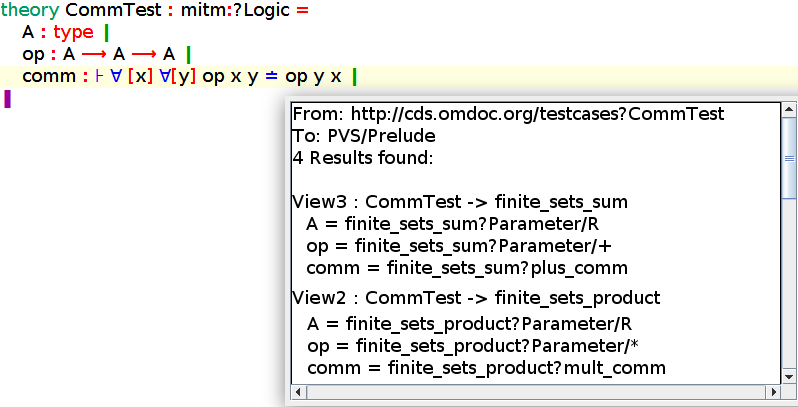
\includegraphics[width=\textwidth]{img/vf-pvs}}
\caption{Searching for Commutative Operators in PVS}\label{fig:use:pvs}
\end{figure}
This example also hints at a way to iteratively improve the results of the view finder: since we can find properties like commutativity and associativity, we can use the results to in turn inform a better normalization of the theory by exploiting these properties. This in turn would potentially allow for finding more views.

To evaluate the approaches to theory parameters we used a simple theory of monoids in the MitM foundation and the theory of monoids in the NASA library as domains for viewfinding with the whole NASA library as target using simple and covariant approaches. The results are summarized in \autoref{fig:pvsresults}.

\begin{figure}[ht]\centering
  \begin{tabular}{l | c || c | c}
  	\textbf{Domain} & \textbf{Normalization} & \textbf{Simple Views} & \textbf{Aggregated} \\\hline\hline
  	NASA/monoid & simple & 388 & 154 \\
  	MitM/monoid & simple & 32 & 17 \\\hline
  	NASA/monoid & covariant & 1026 & 566 \\
  	MitM/monoid & covariant & 22 & 6 \\
  \end{tabular}
\caption{Results of Inter- and Intra-Library View Finding in the PVS NASA Library}\label{fig:pvsresults}
\end{figure}

Most of the results in the simple MitM$\to$NASA case are artifacts of the theory parameter treatment and view amalgamation -- in fact only two of the 17 results are meaningful (to operations on sets and the theory of number fields). In the covariant case, the additional requirements lead to fuller (one total) and less spurious views.
With a theory from the NASA library as domain, the results are already too many to be properly evaluated by hand. With the simple approach to theory parameters, most results can be considered artifacts; in the covariant case, the most promising results yield (partial) views into the theories of semigroups, rings (both the multiplicative and additive parts) and most extensions thereof (due to the duplication of theory parameters as constants).

%%% Local Variables:
%%% mode: latex
%%% eval:  (set-fill-column 5000)
%%% eval:  (visual-line-mode)
%%% TeX-master: "paper"
%%% End:

%  LocalWords:  ednote centering fbox includegraphics textwidth beautysource smglom pvs
%  LocalWords:  newpart Normalization sec:normalizeintra optimizations normalizations a,b
%  LocalWords:  textbf sec:normalizeinter subterms normalizing vdash vdash Rightarrow
%  LocalWords:  vdash vdash vdash forall vdash formalization mathbb sec:usecase coll emph
%  LocalWords:  subtyping PVSlibraries:url monoid formalized pvstype circ,e circ,e ldots
%  LocalWords:  formalizations ldots langle psvtype pvsterm pvsterm pvsterm mmt-term
%  LocalWords:  pvsapply Monoids Monoids summarized fig:pvsresults hline hline
%  LocalWords:  PVSlibraries:on
